
% v2-acmsmall-sample.tex, dated March 6 2012
% This is a sample file for ACM small trim journals
%
% Compilation using 'acmsmall.cls' - version 1.3 (March 2012), Aptara Inc.
% (c) 2010 Association for Computing Machinery (ACM)
%
% Questions/Suggestions/Feedback should be addressed to => "acmtexsupport@aptaracorp.com".
% Users can also go through the FAQs available on the journal's submission webpage.
%
% Steps to compile: latex, bibtex, latex latex
%
% For tracking purposes => this is v1.3 - March 2012
\documentclass[prodmode,acmtecs]{acmsmall} % Aptara syntax
\usepackage[spanish,polish]{babel}
\usepackage[T1]{fontenc}
\usepackage{fancyvrb}
\usepackage{graphicx,hyperref}
\newcommand\cutout[1]{}


\usepackage[table]{xcolor}
\usepackage[utf8]{inputenc}
\usepackage[parfill]{parskip}
\usepackage{tabulary}
\PassOptionsToPackage{hyphens}{url}
\usepackage{hyperref}    
\usepackage[capitalize]{cleveref}


% Metadata Information
% !!! TODO: SET THESE VALUES !!!
\acmVolume{0}
\acmNumber{0}
\acmArticle{CFP}
\acmYear{0}
\acmMonth{0}

\newcounter{colstart}
\setcounter{page}{4}

\RecustomVerbatimCommand{\VerbatimInput}{VerbatimInput}%
{
%fontsize=\footnotesize,
fontfamily=\rmdefault
}


\newcommand{\UnderscoreCommands}{%\do\verbatiminput%
\do\citeNP \do\citeA \do\citeANP \do\citeN \do\shortcite%
\do\shortciteNP \do\shortciteA \do\shortciteANP \do\shortciteN%
\do\citeyear \do\citeyearNP%
}

\usepackage[strings]{underscore}



% Document starts
\begin{document}


\setcounter{colstart}{\thepage}

\acmArticle{CFP}
\title{\huge\sc SIGLOG Monthly 231}
\author{DAVID PURSER\affil{University of Warsaw, Poland}
\vspace*{-2.6cm}\begin{flushright}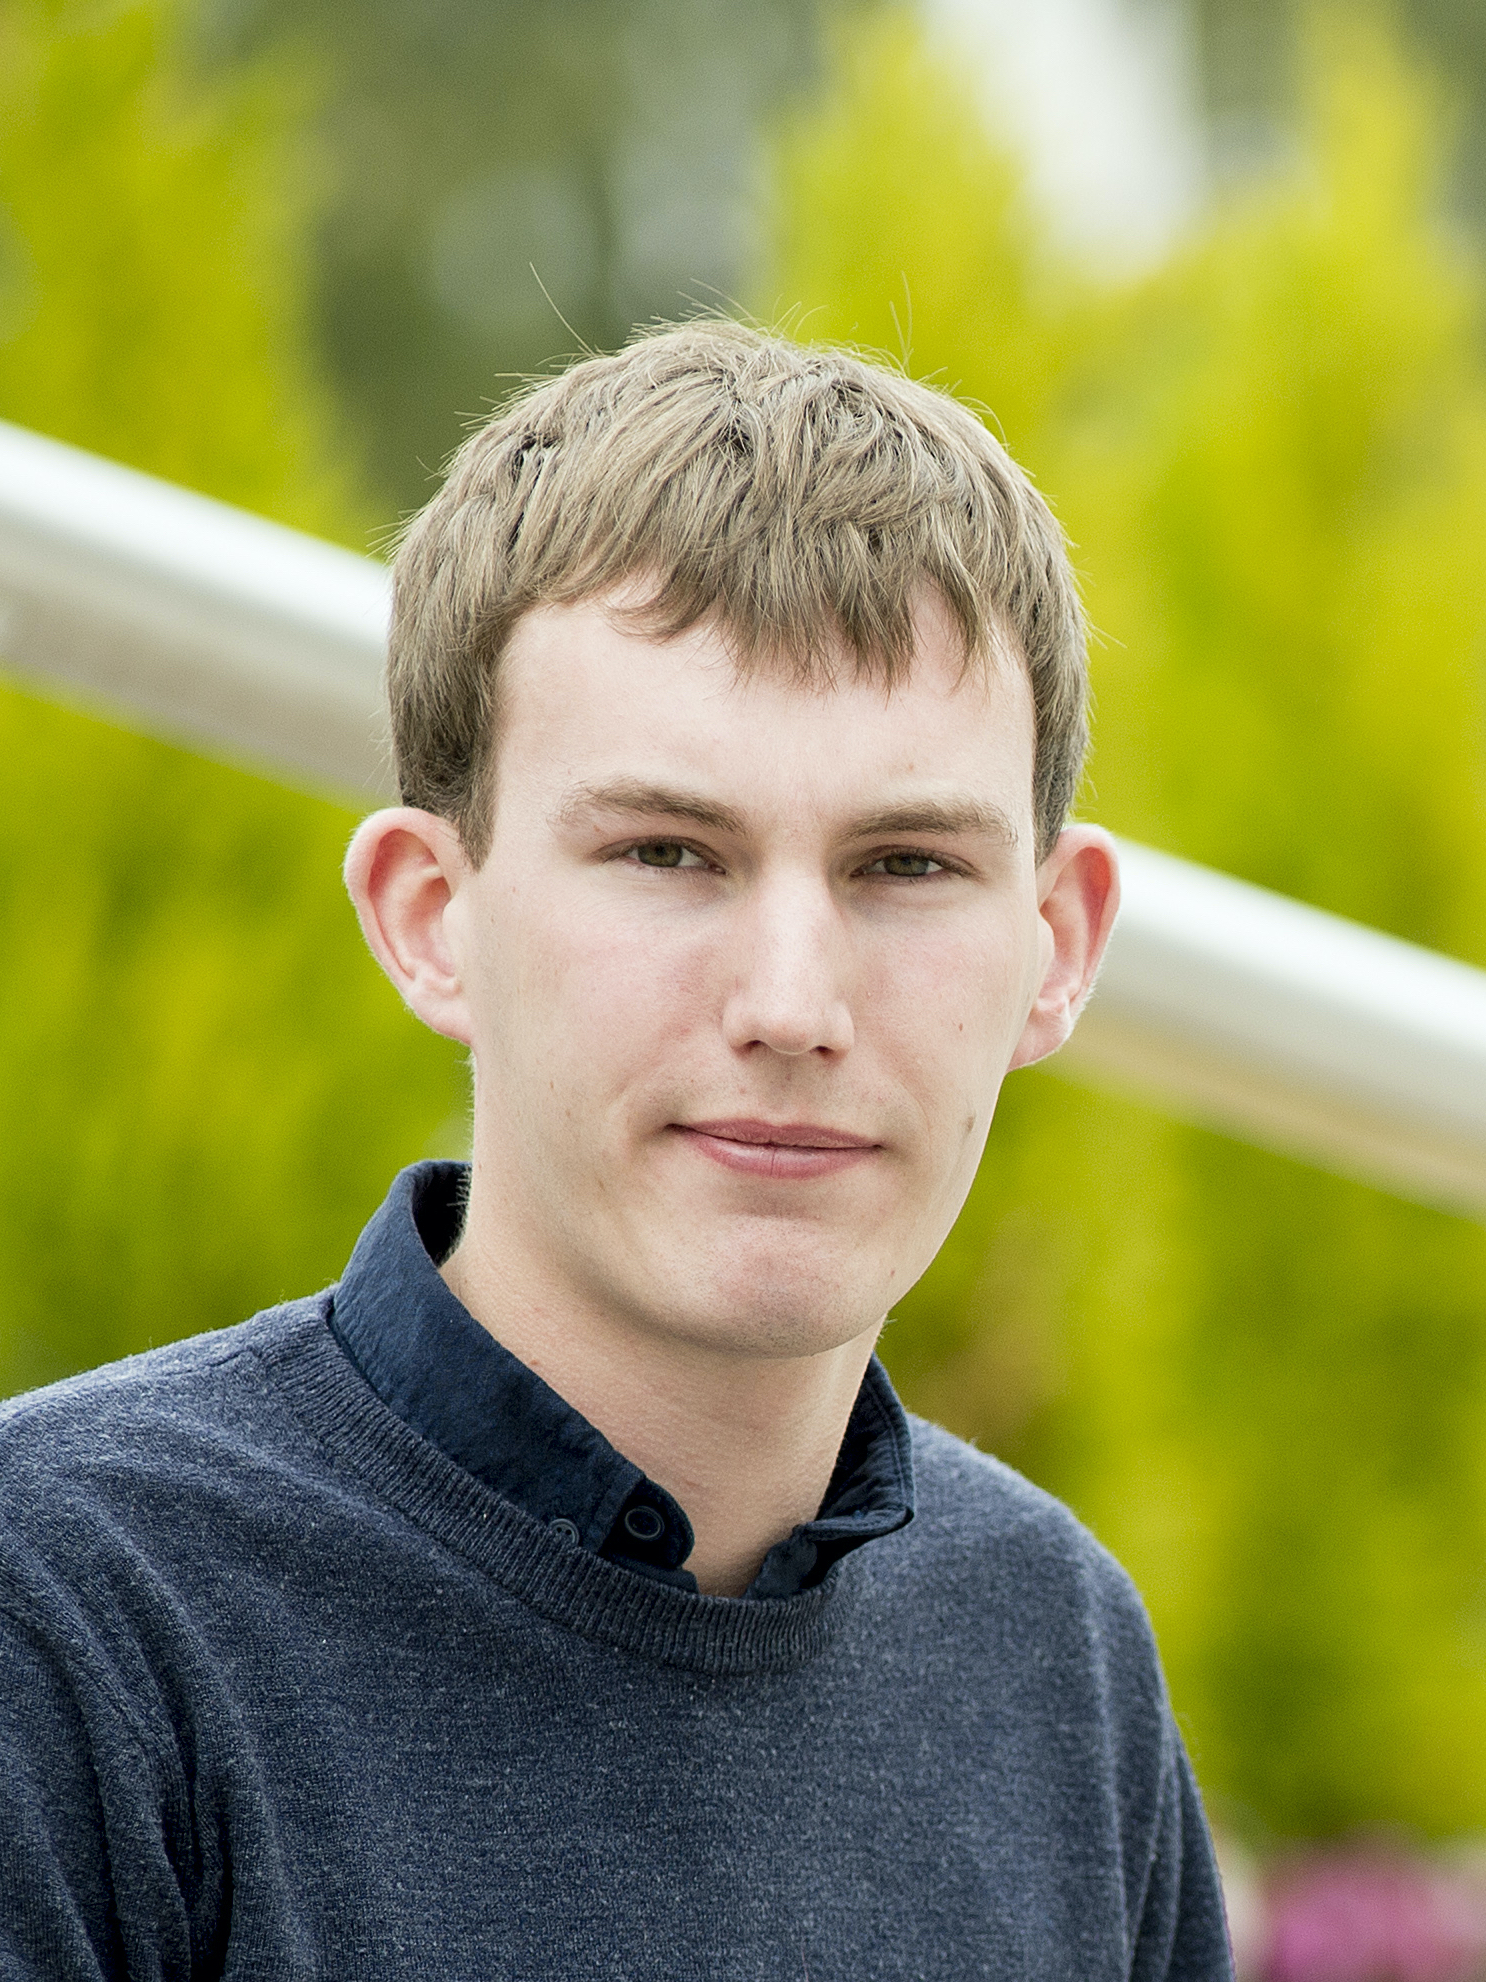
\includegraphics[width=30mm]{dp}\end{flushright}
}

\maketitlee

\href{https://lics.siglog.org/newsletters/}{Past Issues}
 - 
\href{https://lics.siglog.org/newsletters/inst.html}{How to submit an announcement}
\section{Table of Content}\begin{itemize}\item DEADLINES (\cref{deadlines}) 
 
\item SIGLOG MATTERS 
 
\begin{itemize}\item LICS 2023 WORKSHOPS (\cref{LICS2023WORKSHOPS})
\end{itemize} 
\item CALLS 
 
\begin{itemize}\item ACM SIGAI Autonomous Agents Research Award (CALL FOR NOMINATIONS) (\cref{ACMSIGAIAutonomousAgentsResearchAward})
\item Dov Gabbay Prize for Logic and Foundations (CALL FOR NOMINATIONS) (\cref{DovGabbayPrizeforLogicandFoundations})
\item S. Barry Cooper Prize (CALL FOR NOMINATIONS) (\cref{SBarryCooperPrize})
\item CiE 2023 (CALL FOR PAPERS) (\cref{CiE2023})
\item ICALP 2023 (CALL FOR PAPERS) (\cref{ICALP2023})
\end{itemize} 
\item JOB ANNOUNCEMENTS 
 
\begin{itemize}\item Faculty Position at Cambridge (\cref{FacultyPositionatCambridge})
\end{itemize} 
\end{itemize}\section{Deadlines}\label{deadlines}\rowcolors{1}{white}{gray!25}\begin{tabulary}{\linewidth}{LL}FSEN 23:  & Nov 4, 2022 (Extended) \\
TYPES 2022:  & Nov 14, 2022 (Abstract, EXTENDED), Nov 30, 2022 (Paper) \\
ACM SIGAI Autonomous Agents Research Award:  & Nov 15, 2022 (Deadline for nominations) \\
PODS 2023:  & Nov 28, 2022 (Second cycle abstract), Dec 05, 2022 (Full paper) \\
LICS 2023:  & Nov 30, 2022 (Workshop proposals), Jan 18, 2023 (Titles and Short Abstracts Due), Jan 23, 2023 (Full Papers Due) \\
Faculty Position at Cambridge:  & Dec 05, 2022 (Application deadline) \\
Oxford Faculty Positions:  & Dec 14, 2022 at noon (Application deadline) \\
Dov Gabbay Prize for Logic and Foundations:  & Jan 31, 2023 (Deadline for nominations) \\
S. Barry Cooper Prize:  & Jan 31, 2023 (Deadline for nominations) \\
CiE 2023:  & Feb 08, 2023 (Abstract), Feb 15, 2023 (Article) \\
ICALP 2023:  & Feb 11, 2023 at 11am CET (Submissions) \\
\end{tabulary}
\section{LICS 2023 WORKSHOPS: 38TH ANNUAL ACM/IEEE SYMPOSIUM ON LOGIC IN COMPUTER SCIENCE}\label{LICS2023WORKSHOPS}  \href{https://lics.siglog.org/lics23/}{https://lics.siglog.org/lics23/}\\ 
CALL FOR WORKSHOP PROPOSALS 

\begin{itemize}\item  The thirty-eighth Annual ACM/IEEE Symposium on Logic in Computer Science (LICS'23) will be held in Boston, US, on June 26-29, 2023. The workshops will take place on June 24-25, 2023. 
 
\item  Researchers and practitioners are invited to submit proposals for workshops on topics relating logic - broadly construed - to computer science or related fields. Typically, LICS workshops feature a number of invited speakers and a number of contributed presentations. LICS workshops do not usually produce formal proceedings. However, in the past there have been special issues of journals based in part on certain LICS workshops. 
 
\item  Proposals should include: 
 
\begin{itemize}\item   A short scientific summary and justification of the proposed topic. This should include a discussion of the particular benefits of the topic to the LICS community.
\item   Potential invited speakers.
\item   Procedures for selecting participants and papers.
\item   Plans for dissemination (for example, special issues of journals).
\item   The proposed duration, which is one or two days.
\item   A discussion of the proposed format and agenda.
\item   Expected number of participants, providing data on previous years
\end{itemize} 
      if the workshop has already been organised in the past. 
 
  Proposals should be sent to Valentin Blot: lics23-workshops at valentinblot.org 
 
\item  IMPORTANT DATES: 
 
\rowcolors{1}{white}{gray!25}\begin{tabulary}{\linewidth}{LL}Submission deadline:  & Nov 30, 2022 \\
Notification:  & mid-December, 2022 \\
Program of the workshops ready:  & May 24, 2023 \\
Workshops:  & June 24-25, 2023 \\
LICS conference:  & June 26-29, 2023 \\
\end{tabulary}
 
\end{itemize}\section{ACM SIGAI Autonomous Agents Research Award}\label{ACMSIGAIAutonomousAgentsResearchAward}  \href{https://sigai.acm.org/main/the-acm-sigai-autonomous-agents-research-award/}{https://sigai.acm.org/main/the-acm-sigai-autonomous-agents-research-award/}\\ 
CALL FOR NOMINATIONS 

\begin{itemize}\item   Nominations are solicited for the 2023 ACM SIGAI Autonomous Agents Research Award. This award is made for excellence in research in the area of autonomous agents. It is intended to recognize researchers in autonomous agents whose current work is an important influence on the field. The award is an official ACM award, funded by an endowment created by ACM SIGAI from the proceeds of previous Autonomous Agents conferences. The recipient of the award will receive a monetary prize and a certificate, and will be invited to present a plenary talk at the AAMAS 2023 conference in London, United Kingdom. 
 
\item  How to Nominate 
 
  Anyone can make a nomination. Nominations should be made by email to the chair of the award committee, Manuela Veloso (mmv@cs.cmu.edu), and should consist of a short (< 1 page) statement that emphasizes not only the research contributions that the individual has made that merit the award but also how the individual’s current work is an important influence on the field. 
 
  NOTE: a candidate can only be considered for the award if they are explicitly nominated. If you believe that someone deserves the award, then NOMINATE THEM — don’t assume that somebody else will! 
 
\item  IMPORTANT DATES 
 
\rowcolors{1}{white}{gray!25}\begin{tabulary}{\linewidth}{LL}Deadline for nominations:  & Nov 15, 2022 \\
Announcement of winner:  & Dec 15, 2022 \\
AAMAS-2023 conference in London, United Kingdom:  & May 29-Jun 2, 2023 \\
\end{tabulary}
 
\end{itemize}\section{Dov Gabbay Prize for Logic and Foundations}\label{DovGabbayPrizeforLogicandFoundations}  Deadline: Jan 31, 2023\\ 
CALL FOR NOMINATIONS 

\begin{itemize}\item  THE PRIZE 
 
  The ``Dov Gabbay Prize for Logic and Foundations'' is an international research prize established to honour the extraordinary, multi-faceted, and ongoing scientific and editorial work of Prof. Dov Gabbay, known in particular for editing an extensive collection of specialized Logic Handbooks. It has been launched on the occasion of his 77th birthday (for a short bio, see: \href{https://dgp.iloaf.org/dov.html}{https://dgp.iloaf.org/dov.html}). 
 
  The prize rewards outstanding researchers in Logic and Foundations, including Mathematical, Philosophical, and Computational Logic. It promotes work able to inspire current and future generations of logicians, if not a broader audience, ideally combining deep foundational insight and conceptual innovation with sophisticated theoretical analysis. 
 
  The winner will receive 2001 EUR and be invited to give a talk (accessible for an online audience) at a major logic centre or a logic-related meeting in 2023, the choice depending on the recipient's research area. Additional efforts will be made to promote the rewarded scientific work. 
 
\item  NOMINATION 
 
  Each nomination has to specify the researcher, provide a justification accessible to non-expert logicians (0.5-2 pages), and list the publications considered relevant. 
 
  It also has to include the name, affiliation, and email address of the nominator. Self-nominations are not allowed, the nominator should not depend on the nominee. 
 
  Proposals in pdf-format have to be sent to ``dgp@iloaf.org''.  
 
  The deadline for this call is Jan 31, 2023. 
 
\item  DECISION 
 
  The decision is made by an independent selection committee consisting of six internationally renowned logicians representing Mathematical, Philosophical, and Computational logic (for details, see: \href{https://dgp.iloaf.org}{https://dgp.iloaf.org}). The jury can decide to attribute no prize in a given year. The winner of the 2022 call will be announced in May 2023. 
 
\item  ADMIN 
 
  Prize and process are managed by the ``Logic and Foundations Initiative (ILOAF)'', which aims at initiating and supporting scientific and educational activities in Logic and Foundations. It is currently sponsored by the Luxembourg Logic Community. 
 
\item  CONTACT 
 
  For any questions, please contact the organizing committee (only) via email. 
 
  Web: \href{https://dgp.iloaf.org}{https://dgp.iloaf.org}  
 
  Email: dgp@iloaf.org 
 
\end{itemize}\section{S. Barry Cooper Prize}\label{SBarryCooperPrize}  Association Computability in Europe\\ 
  Deadline: Jan 31, 2023\\ 
  \href{https://www.acie.eu/2022/10/03/call-for-nominations-for-2023-s-barry-cooper-prize/}{https://www.acie.eu/2022/10/03/call-for-nominations-for-2023-s-barry-cooper-prize/}\\ 
CALL FOR NOMINATIONS 

  The S. Barry Cooper Prize is awarded to a researcher who has contributed to a broad understanding and foundational study of computability by outstanding results, by seminal and lasting theory building, by exceptional service to the research communities involved, or by a combination of these. This award is presented every two to three years, with the presentation taking place at the International Conference Computability in Europe (CiE).\\ 
  The Prize is named in honor of S. Barry Cooper, the founding President of the Association Computability, in recognition of his vision of the fundamental concept of computability that brought together several different research communities. The awardee shall be invited to the next annual CiE conference to give an invited talk and will be presented with an award plaque on this occasion.\\ 
\begin{itemize}\item  NOMINATIONS AND ELIGIBILITY 
 
  Nominations may be made by any member of the scientific community and any such member can be nominated. Nomination letters can have multiple signatories and should provide a motivation for awarding the prize to the nominee, precisely stating their outstanding results, their seminal and lasting theory building, and/or their exceptional service to the research communities involved. 
 
  Nominations for the award should be submitted by email to the Award Committee Chair: 
 
\begin{itemize}\item  Anuj Dawar (University of Cambridge) anuj.dawar@cl.cam.ac.uk
\end{itemize} 
  Any emails and related messages should have the subject line starting with “S. Barry Cooper Prize 2023”. 
 
  To be considered, nominations for the 2023 Prize must be received by Jan 31, 2023. 
 
  A nomination package should include: 
 
  1. A statement of motivation for awarding the prize to the nominee describing the nominee’s outstanding results, their seminal and lasting theory building and/or exceptional service to the research communities, as the case may be. These should be supported by at least one of 
 
\begin{itemize}\item  A list of the most important publications, accompanied by a brief summary of the technical content of the papers and a brief explanation of their significance. Where possible, this should include pointers to online versions of the publications.
\item  A statement explaining the role played and the exceptional services rendered by the nominee, in the research communities involved in computability and related areas.
\end{itemize} 
  2. A support letter or letters signed by at least two members of the scientific community. The nomination package must be in English, but it may include reference to publications in other languages. 
 
\item  Selection Process 
 
  The Award Committee is solely responsible for the selection of the winner of the award. All matters relating to the selection process that are not specified here are left to the discretion of the Award Committee, whose decision will be final. 
 
\end{itemize}\section{CiE 2023: Computability in Europe 2023}\label{CiE2023}  Batumi, Georgia\\ 
  July 24-28, 2023\\ 
  \href{https://www.viam.science.tsu.ge/cie2023/}{https://www.viam.science.tsu.ge/cie2023/}\\ 
CALL FOR PAPERS 

\begin{itemize}\item  IMPORTANT DATES: (AOE) 
 
\rowcolors{1}{white}{gray!25}\begin{tabulary}{\linewidth}{LL}Abstract submission:  & Feb 08, 2023 \\
Article submission:  & Feb 15, 2023 \\
Notification of acceptance:  & Apr 20, 2023 \\
Final versions due:  & May 01, 2023 \\
Deadline for informal presentations submission:  & Jun 8, 2023 (The notifications of acceptance for informal presentations will be sent a few days after submission.) \\
Early registration before:  & Jun 10, 2023 \\
\end{tabulary}
 
\item  GENERAL INFORMATION 
 
  CiE 2023 is the 19th conference organized by CiE (Computability in Europe), a European association of mathematicians, logicians, computer scientists, philosophers, physicists and others interested in new developments in computability and their underlying significance for the real world. 
 
\item  TUTORIAL SPEAKERS 
 
\begin{itemize}\item  Ludovic Perret (Sorbonne University)
\item  Ludovic Patey (Université Paris Diderot)
\end{itemize} 
\item  INVITED SPEAKERS;  
 
  Andrei Bulatov (Simon Fraser University); Anne Condon (University of British Columbia); Stephanie Dick (University of Pennsylvania); Kirsten Eisenträger (Pennsylvania State University); Neil Lutz (Iowa State University); Mark Steedman (University of Edinburgh) 
 
\item  SPECIAL SESSIONS 
 
  We are going to have 6 special sessions. The topics of the special sessions will be announced soon. 
 
\item  CONFERENCE TOPICS 
 
  The CiE conferences serve as an interdisciplinary forum for research in all aspects of computability, foundations of computer science, logic, and theoretical computer science, as well as the interplay of these areas with practical issues in computer science and with other disciplines such as biology, mathematics, philosophy, or physics. 
 
\item  PAPER SUBMISSION 
 
  THE PROGRAM COMMITTEE cordially invites all researchers, European and non-European, to submit their papers in all areas related to the above for presentation at the conference and inclusion in the proceedings of CiE 2023 at \href{https://easychair.org/conferences/?conf=cie2023}{https://easychair.org/conferences/?conf=cie2023} 
 
  CONFERENCE PROCEEDINGS   
 
\begin{itemize}\item  Papers submitted to the conference proceedings should represent original work, not simultaneously submitted to another journal or conference with formal proceedings.
\item  The Program Committee will rigorously review and select submitted papers. Accepted papers will be published as a proceedings volume in the Lecture Notes in Computer Science (LNCS) series from Springer-Verlag.
\item  Papers to be considered in the conferences proceedings must be submitted in PDF format, using the LNCS style (available at \href{https://www.springer.com/gp/computer-science/lncs/conference-proceedings-guidelines}{https://www.springer.com/gp/computer-science/lncs/conference-proceedings-guidelines}) and must have a maximum of 12 pages, including references but excluding a possible appendix in which one can include proofs and other additional material. Papers building bridges between different parts of the research community are particularly welcome.
\end{itemize} 
  INFORMAL PRESENTATIONS 
 
\begin{itemize}\item  Continuing the tradition of past CiE conferences, we invite researchers to present informal presentations of their recent work. A proposal for an informal presentation must be submitted via EasyChair (\href{https://easychair.org/conferences/?conf=cie2023}{https://easychair.org/conferences/?conf=cie2023}), using the LNCS style file (available at \href{https://www.springer.com/gp/computer-science/lncs/conference-proceedings-guidelines}{https://www.springer.com/gp/computer-science/lncs/conference-proceedings-guidelines}), and be 1 page long; a brief description of the results suffices and an abstract is not required. Informal presentations will not be published in the LNCS conference proceedings. Results presented as informal presentations at CiE 2023 may appear or may have appeared in other conferences with formal proceedings and/or in journals.
\end{itemize} 
\end{itemize}\section{ICALP 2023: The 50th EATCS International Colloquium on Automata, Languages, and Programming}\label{ICALP2023}  Paderborn, Germany, 10-14 July 2023.\\ 
  \href{https://icalp2023.cs.upb.de/}{https://icalp2023.cs.upb.de/}\\ 
  Twitter: @ICALPconf\\ 
CALL FOR PAPERS 

\begin{itemize}\item  ABOUT 
 
  ICALP is the main conference and annual meeting of the European Association for Theoretical Computer Science (EATCS). As usual, ICALP will be preceded by a series of workshops, which will take place on July 10. The 2023 edition has the following features: 
 
\begin{itemize}\item  Submissions are anonymous, and there is a rebuttal phase.
\item  The conference is planned as a physical, in-person event.
\item  This will be the 50th ICALP conference and some special events are planned.
\end{itemize} 
\item  IMPORTANT DATES AND INFORMATION 
 
\rowcolors{1}{white}{gray!25}\begin{tabulary}{\linewidth}{LL}Submissions:  & Feb 11, 2023 at 11am CET \\
Rebuttal:  & Mar 22-25, 2023 \\
Author notification:  & Apr 21, 2023 \\
Camera-ready version:  & May 05, 2023 \\
Early registration:  & TBA \\
Conference:  & Jul 10-14, 2023 (Workshops on July 10, 2023) \\
\end{tabulary}
 
  Deadlines are firm; late submissions will not be considered. 
 
\item  INVITED SPEAKERS 
 
\begin{itemize}\item  Anna Karlin - University of Washington, USA
\item  Rasmus Kyng - ETH Zurich, Switzerland
\item  Rupak Majumdar - Max Planck Institute for Software Systems, Germany
\item  Thomas Vidick - California Institute of Technology, USA, and Weizmann Institute of Science, Israel
\item  James Worrell - University of Oxford, UK
\end{itemize} 
\item  SUBMISSION GUIDELINES 
 
  15 page (excl. references+appendix), PDF in LIPIcs format, anonymous/double-blind, original research with no concurrent submission, submission via EasyChair: \href{https://easychair.org/conferences/?conf=icalp2023}{https://easychair.org/conferences/?conf=icalp2023} 
 
  See full call for full rules and guidance: \href{https://icalp2023.cs.upb.de/call-for-papers/}{https://icalp2023.cs.upb.de/call-for-papers/} 
 
  Resulting publications will be open access via LIPIcs. 
 
\item  AWARDS 
 
  During the conference, the following awards will be given: 
 
\begin{itemize}\item  the EATCS award,
\item  the Church prize,
\item  the Presburger award,
\item  the EATCS distinguished dissertation award,
\item  the best papers for Track A and Track B,
\item  the best student papers for Track A and Track B (see submission guidelines).
\end{itemize} 
\item  TOPICS 
 
  Papers presenting original research on all aspects of theoretical computer science are sought. Typical but not exclusive topics of interest are: 
 
\begin{itemize}\item  Track A: Algorithms, Complexity and Games: Algorithmic and Complexity Aspects of Network Economics; Algorithmic Aspects of Biological and Physical Systems; Algorithmic Aspects of Networks and Networking; Algorithmic Aspects of Security and Privacy; Algorithmic Game Theory and Mechanism Design; Approximation and Online Algorithms; Combinatorial Optimization; Combinatorics in Computer Science; Computational Complexity; Computational Geometry; Computational Learning Theory; Cryptography; Data Structures; Design and Analysis of Algorithms; Distributed and Mobile Computing; Foundations of Machine Learning; Graph Mining and Network Analysis; Parallel and External Memory Computing; Parameterized Complexity; Quantum Computing; Randomness in Computation; Sublinear Time and Streaming Algorithms; Theoretical Foundations of Algorithmic Fairness
\item  Track B: Automata, Logic, Semantics, and Theory of Programming: Algebraic and Categorical Models of Computation; Automata, Logic, and Games; Database Theory, Constraint Satisfaction Problems, and Finite Model Theory; Formal and Logical Aspects of Learning; Formal and Logical Aspects of Security and Privacy; Logic in Computer Science and Theorem Proving; Models of Computation: Complexity and Computability; Models of Concurrent, Distributed, and Mobile Systems; Models of Reactive, Hybrid, and Stochastic Systems; Principles and Semantics of Programming Languages; Program Analysis, Verification, and Synthesis; Type Systems and Typed Calculi
\end{itemize} 
\end{itemize}\section{Faculty Position at Cambridge}\label{FacultyPositionatCambridge}  \href{https://www.jobs.cam.ac.uk/job/37369/}{https://www.jobs.cam.ac.uk/job/37369/}\\ 
JOB ANNOUNCEMENT 

\begin{itemize}\item  Assistant/Associate Professor in Logical Foundations and Formal Methods in the Department of Computer Science and Technology, University of Cambridge 
 
\item  The Department is seeking to recruit a new faculty member at the Assistant or Associate Professor level who can contribute to research and teaching in the area of Logical Foundations and Formal Methods. 
 
\item  DATE 
 
Application deadline: Dec 05, 2022 
 
\item  Interested applicants are encouraged to make informal enquiries about the post to marcelo.fiore@cl.cam.ac.uk 
 
\end{itemize}


To the \href{http://siglog.org/}{SIGLOG} or \href{https://lics.siglog.org}{LICS} website\end{document}